%\VignetteIndexEntry{HTShape: Shape analysis of high-throughput experiments data}
%\VignetteEngine{knitr::knitr}
%\VignetteDepends{HTShape}

\documentclass[a4paper, 10pt]{article}\usepackage[]{graphicx}\usepackage[]{color}
%% maxwidth is the original width if it is less than linewidth
%% otherwise use linewidth (to make sure the graphics do not exceed the margin)
\makeatletter
\def\maxwidth{ %
  \ifdim\Gin@nat@width>\linewidth
    \linewidth
  \else
    \Gin@nat@width
  \fi
}
\makeatother

\definecolor{fgcolor}{rgb}{0.345, 0.345, 0.345}
\newcommand{\hlnum}[1]{\textcolor[rgb]{0.686,0.059,0.569}{#1}}%
\newcommand{\hlstr}[1]{\textcolor[rgb]{0.192,0.494,0.8}{#1}}%
\newcommand{\hlcom}[1]{\textcolor[rgb]{0.678,0.584,0.686}{\textit{#1}}}%
\newcommand{\hlopt}[1]{\textcolor[rgb]{0,0,0}{#1}}%
\newcommand{\hlstd}[1]{\textcolor[rgb]{0.345,0.345,0.345}{#1}}%
\newcommand{\hlkwa}[1]{\textcolor[rgb]{0.161,0.373,0.58}{\textbf{#1}}}%
\newcommand{\hlkwb}[1]{\textcolor[rgb]{0.69,0.353,0.396}{#1}}%
\newcommand{\hlkwc}[1]{\textcolor[rgb]{0.333,0.667,0.333}{#1}}%
\newcommand{\hlkwd}[1]{\textcolor[rgb]{0.737,0.353,0.396}{\textbf{#1}}}%

\usepackage{framed}
\makeatletter
\newenvironment{kframe}{%
 \def\at@end@of@kframe{}%
 \ifinner\ifhmode%
  \def\at@end@of@kframe{\end{minipage}}%
  \begin{minipage}{\columnwidth}%
 \fi\fi%
 \def\FrameCommand##1{\hskip\@totalleftmargin \hskip-\fboxsep
 \colorbox{shadecolor}{##1}\hskip-\fboxsep
     % There is no \\@totalrightmargin, so:
     \hskip-\linewidth \hskip-\@totalleftmargin \hskip\columnwidth}%
 \MakeFramed {\advance\hsize-\width
   \@totalleftmargin\z@ \linewidth\hsize
   \@setminipage}}%
 {\par\unskip\endMakeFramed%
 \at@end@of@kframe}
\makeatother

\definecolor{shadecolor}{rgb}{.97, .97, .97}
\definecolor{messagecolor}{rgb}{0, 0, 0}
\definecolor{warningcolor}{rgb}{1, 0, 1}
\definecolor{errorcolor}{rgb}{1, 0, 0}
\newenvironment{knitrout}{}{} % an empty environment to be redefined in TeX

\usepackage{alltt}
\usepackage{url}
\usepackage{afterpage}
\usepackage{hyperref}
\usepackage{geometry}
\usepackage{cite}
\geometry{hmargin=2.5cm, vmargin=2.5cm}
\usepackage{graphicx}
\usepackage{courier}
\bibliographystyle{unsrt}
\IfFileExists{upquote.sty}{\usepackage{upquote}}{}
\begin{document}

% Define global R and R chunk options.


\title{{\textbf{\texttt{HTShape}}: Shape analysis of high-throughput experiments data}}

\author{Kwame Okrah${}^{*}$,  H\'ector Corrada-Bravo \\\\\ 
        Applied Mathematics, Statistics, and Scientific Computation \\ 
        Center for Bioinformatics and Computational Biology \\ 
        University of Maryland, College Park \\\\ 
        \texttt{${}^{*}$kwame.okrah (at) gmail.com}}

\date{\today}

\maketitle

\begin{abstract}
\normalsize
Given a dataset we first try to characterize 
its central value (location) with the sample 
mean (or sample median) and its spread around 
the location (variance) with the sample standard 
deviation (or sample range).
When the sample size, $n$, is sufficiently 
large we can begin to assess the shape of the 
data in some meaningful way. 
Distributional shape is often characterized by 
two features 
(1) Skewness: a measure of how far the
shape of the distribution deviates from symmetry
around its location and 
(2) Kurtosis: a measure of how much
weight is at the tails of the distribution relative 
to the weight around the location.
This vignette describes the statistical 
analysis of the shape (skewness and kurtosis)
of high-throughput experiments data 
(e.g. RNA-seq, microarry) using the 
\textbf{\texttt{shape}} package. 
It also demonstrates the detection of 
transcripts (e.g. genes) within a dataset
whose sample shape is markedly different from 
the majority of transcripts in the same dataset. 
The ability to describe the shape of high-throughput
genomics data is useful for two reasons: 
1. It enriches the exploratory data analysis process, and
2. It provides a means of checking the distributional 
assumptions of statistical methods.
\end{abstract}

\vspace{1 cm}

\noindent \underline{If you use 
\textbf{\texttt{HTShape}} 
(version 1.0.0) 
in your work, please cite:}

\renewcommand\refname{\vskip -1cm} 

\begin{thebibliography}{9}

\makeatletter
\renewcommand\@biblabel[1]{\textbullet}
\makeatother

\bibitem{shapePaper} K. Okrah and H. Bravo. 
         \emph{HTShape analysis of high-throughput experiments data.}  
         Under review.
         
\bibitem{hosking} J. Hosking. 
         \emph{L-moments: analysis and estimation 
               of distributions using linear 
               combinations of order statistics.}    
               Journal of the Royal Statistical Society. 
               Series B (Methodological),
               \textbf{52}, 105--124, 1990.                 
               
\bibitem{okrah} K. Okrah.
          \texttt{shape}: Shape analysis of high-throughput 
          experiments data. 
          R package version 1.0.0,
          2014 (\url{https://github.com/kokrah/HTShape}).
          
\end{thebibliography}

\newpage

\tableofcontents

\newpage

\section{Introduction}

Before we begin we first give a brief
description of the theory on which
our methods are based.

\subsection{A numerical summary of shape}

\noindent Similar to traditional moments,
the theory of L-moments
forms the basis of many statistical methods 
such as parameter estimation, hypothesis testing, 
and model selection. However, L-moments enjoy 
many theoretical and practical advantages over
traditional moments 
(see \cite{Kirby1974, Hosking1990, Vogel1993, Delicado2008}).
In this vignette we focus on its ability to
provide robust statistics that summarize a given 
dataset.
The first four L-moments $\lambda_1, \lambda_2, \lambda_3$ 
and $\lambda_4$ measure location, variance,
skewness, and kurtosis of data respectively. 
Unit free measures of relative variance, skewness,
and kurtosis are defined as: 
L-CV $\tau = \lambda_2 / \lambda_1$, 
L-skew $\tau_3 = \lambda_3 / \lambda_2$,
and 
L-kurt $\tau_4 = \lambda_4 / \lambda_2$.
The L-skew ($\tau_3$) coefficient can take any
value between (-1, 1); where $\tau_3=0$ implies symmetry
and $\tau_3 > 0$ ($\tau_3 < 0$) implies skewness to 
the right (left).
The symmetry-outlier plot (SO-plot) 
conveniently summarizes the shape of each gene as a point
on a 2-dimensional plot 
(see L-moments ratio diagram in \cite{Hosking1990}).
The interpretation of the L-kurt ($\tau_4$) 
depends on L-skew (in general one would expect a 
highly skewed data to have a high kurtosis).
At $\tau_3 = 0$ and $\tau_4 = 0$ the data has the shape 
of a uniformly distributed random variable.
As $\tau_4$ (positive) increases the data becomes bell
shaped, for example at $\tau_4 = 0.1226$ the data is 
normally distributed. 
As $\tau_4$ (negative) decreases the data becomes 
U-shaped (indicating two possible groups). 
See Figure \ref{interpret} below for examples. 

\begin{figure}[!h]
\centerline{\resizebox{0.75\textwidth}{!}{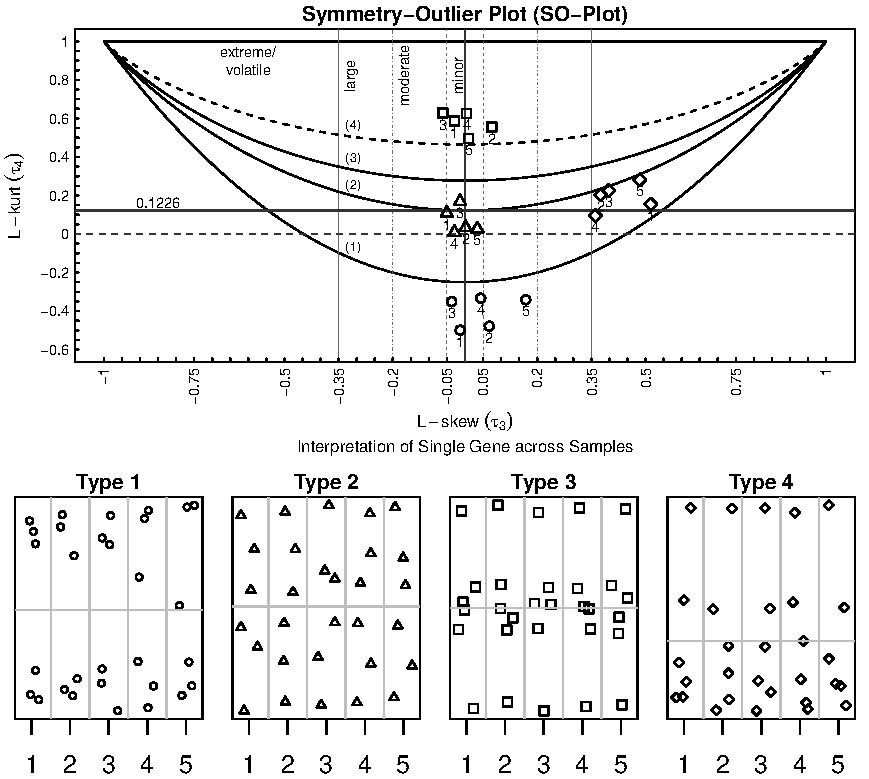
\includegraphics{interpret.pdf}}}
\caption{{\bf Interpretation of the SO-plot.}
       We have shown examples, 
       based on a sample of size 6, of the 
       four main types of sample shape
       (bottom panels) and where they
       occur on the SO-plot (top panel).
       Every single point on the SO-plot corresponds
       to a summary of the shape of a single 
       gene.
       The measure of skewness and kurtosis 
       are not independent, as one would 
       expect a highly skewed sample would
       tend to have a high kurtosis.
       This relationship is indicated by 
       the parabolas on the SO-plot.
       Starting from below:
       (1) we have the theoretical lower
       bound for L-kurt, in terms of L-skew,
       $\tau_4 = 0.25 (5\tau^2_3 - 1)$.
       Between the second (2) and third (3)
       parabolas is a region where the 
       L-kurt measure is considered moderate.
       Between the third (3) and fourth (4)
       parabolas indicate a region where 
       the L-kurt measure is considered to be high. 
       Above the fourth curve is considered extreme.
       One should keep in mind that these descriptive 
       measures are independent of the expression level and
       variance of the gene. Interpretation of the 
       SO-plot ultimately rests on the context of the data.}
\label{interpret}
\end{figure}


\subsection{Package overview}

The purpose of this package is to compute
the shape statistics of each gene in a high-throughput dataset.
Using these statistics we can find
genes within a dataset
whose sample shape is markedly different from 
the majority of genes in the same dataset. 
When put together these shape statistics give an overall
description of the entire high-throughput dataset.
The ability to describe the shape of high-throughput
genomics data is useful for two reasons: 
1. It enriches the exploratory data analysis step, and
2. It provides a means of checking the distributional 
assumptions of statistical methods.\\

\noindent There are three main functions in the \textbf{\texttt{shape}} 
package:
\begin{enumerate}
\item \texttt{fitShape()}
\item \texttt{computeDvals()}
\item \texttt{plotSO()}
\end{enumerate}

\noindent Given a dataset such as a high-throughput expression matrix 
(or just a vector of measurements) the function \texttt{fitShape()}
will compute and return the L-CV, L-skew, and L-kurt estimates 
for each gene.\\

\noindent Given the shape (i.e. L-skew and L-kurt) estimate
of each gene, the function 
\texttt{computeDvals()} computes a dissimilarity 
distance (d-values) between each gene's shape estimate
and the typical gene's shape estimate. 
The d-values range from 0 to 1; where 1 is very close and 
0 is very far.\\  

\noindent The function \texttt{plotSO()} shows 
each gene's shape estimate on a single plot (SO-plot). 

\subsection{Vignette overview}

We will demonstrate the utility of the \textbf{\texttt{shape}}
package as part of the data exploratory steps in the analysis of 
high-throughput experiments data. 
A total of three publicly available datasets will
be used in this vignette :

\begin{enumerate}
\item The \textbf{Pickrell dataset}  
      \cite{Pickrell2010}
      is part of the International 
      HapMap Project. 
      RNA samples were extracted from
      the lymphoblastoid cell lines of 69 
      unrelated Nigerian 
      individuals, 29 males and 40 females. 
      See \cite{Frazee2011} for details on alignment 
      and counting. 
\item The \textbf{Hammoud dataset} \cite{Hammoud2014}
      contains 10 samples of mRNA samples of 8-week 
      old wild type mice (strain: C57BL/6). 
      Of the 10 RNA samples 5 were obtained from
      spermatids (cells) and the other 5
      from spermatocytes (cells).
      Summarized counts in the form 
      of FPKM can be downloaded at 
      GEO:GSE49622.
      For the details on alignment and counting
      please see \cite{Hammoud2014}. 
\item The \textbf{Bottomly dataset} \cite{Bottomly2011}
      was obtained from the ReCount webpage. 
      See \cite{Frazee2011} for details on alignment 
      and counting.
      It contains counts summarizing an RNA-seq 
      experiment that includes 21 samples from
      inbred mouse strains.
      Eleven of the samples came from the strain DBA/2J
      and 10 from the strain C57BL/6J. 
\end{enumerate}

\newpage

\section{The Pickrell dataset}

The datasets in this package are bundled together 
in the form of a list. 
Each component of the list contains the 
expression measures and its experimental design.
We will use the Pickrell dataset to illustrate
the main functions in this package.\\

\noindent We begin by loading the \textbf{\texttt{shape}} 
package into an \texttt{R} session and looking at the
datasets available in the package.

\begin{knitrout}\small
\definecolor{shadecolor}{rgb}{0.969, 0.969, 0.969}\color{fgcolor}\begin{kframe}
\begin{alltt}
\hlstd{> }\hlkwd{library}\hlstd{(HTShape)}
\hlstd{> }\hlkwd{data}\hlstd{(examplesData)} \hlcom{# Load datasets.}
\hlstd{> }\hlkwd{names}\hlstd{(examplesData)}
\end{alltt}
\begin{verbatim}
[1] "bottomly" "hammoud"  "pickrell"
\end{verbatim}
\end{kframe}
\end{knitrout}

\subsection{Filter counts and normalize}

First we will filter out genes with low 
expression by only keeping genes whose
counts per million (cpm) is more than 1 in 
at least 29 samples (where 29 is the minimum of
the 29 male samples and 40 female samples).\\

\noindent Let us define a function to filter
out the low count genes

\begin{knitrout}\small
\definecolor{shadecolor}{rgb}{0.969, 0.969, 0.969}\color{fgcolor}\begin{kframe}
\begin{alltt}
\hlstd{> }\hlstd{filterCounts} \hlkwb{<-} \hlkwa{function} \hlstd{(}\hlkwc{pcounts}\hlstd{,} \hlkwc{thresh}\hlstd{,} \hlkwc{minSamples}\hlstd{) \{}
\hlstd{ }  \hlstd{cpm} \hlkwb{<-} \hlkwd{t}\hlstd{(}\hlkwd{t}\hlstd{(pcounts)} \hlopt{/}  \hlkwd{colSums}\hlstd{(pcounts))} \hlopt{*} \hlnum{1e+06}
\hlstd{ }  \hlstd{keep} \hlkwb{<-} \hlkwd{rowSums}\hlstd{(cpm} \hlopt{>} \hlstd{thresh)} \hlopt{>=} \hlstd{minSamples}
\hlstd{ }  \hlstd{filteredPcounts} \hlkwb{<-} \hlstd{pcounts[keep, ]}
\hlstd{ }  \hlstd{filteredPcounts}
\hlstd{ }\hlstd{\}}
\end{alltt}
\end{kframe}
\end{knitrout}

\noindent and apply it to the Pickrell dataset.

\begin{knitrout}\small
\definecolor{shadecolor}{rgb}{0.969, 0.969, 0.969}\color{fgcolor}\begin{kframe}
\begin{alltt}
\hlstd{> }\hlstd{counts} \hlkwb{<-} \hlstd{examplesData}\hlopt{$}\hlstd{pickrell}\hlopt{$}\hlstd{exprs}
\hlstd{> }\hlstd{gender} \hlkwb{<-} \hlstd{examplesData}\hlopt{$}\hlstd{pickrell}\hlopt{$}\hlstd{cond}
\hlstd{> }\hlstd{(tab} \hlkwb{<-} \hlkwd{table}\hlstd{(gender))}
\end{alltt}
\begin{verbatim}
gender
female   male 
    40     29 
\end{verbatim}
\begin{alltt}
\hlstd{> }\hlstd{pcounts} \hlkwb{<-} \hlstd{counts} \hlopt{+} \hlnum{1} \hlcom{# pseudo-counts}
\hlstd{> }\hlstd{minSamples} \hlkwb{<-} \hlkwd{min}\hlstd{(tab)}
\hlstd{> }\hlkwd{dim}\hlstd{(pcounts)} \hlcom{# Before filtration.}
\end{alltt}
\begin{verbatim}
[1] 38415    69
\end{verbatim}
\begin{alltt}
\hlstd{> }\hlstd{pcounts} \hlkwb{<-} \hlkwd{filterCounts}\hlstd{(pcounts,} \hlnum{1}\hlstd{, minSamples)}
\hlstd{> }\hlkwd{dim}\hlstd{(pcounts)} \hlcom{# After filtration. }
\end{alltt}
\begin{verbatim}
[1] 17604    69
\end{verbatim}
\end{kframe}
\end{knitrout}

\noindent After filtration we normalize for 
library size and transform the data to 
$\hbox{log}_2$ scale. In this vignette we use the DEseq method 
\cite{Anders2010}, however any of the 
library size normalization methods can be used.

\begin{knitrout}\small
\definecolor{shadecolor}{rgb}{0.969, 0.969, 0.969}\color{fgcolor}\begin{kframe}
\begin{alltt}
\hlstd{> }\hlstd{ref} \hlkwb{<-} \hlkwd{exp}\hlstd{(}\hlkwd{rowMeans}\hlstd{(}\hlkwd{log}\hlstd{(pcounts)))}
\hlstd{> }\hlstd{deseqScal} \hlkwb{<-} \hlkwd{apply}\hlstd{(pcounts} \hlopt{/} \hlstd{ref,} \hlnum{2}\hlstd{, median)}
\hlstd{> }\hlstd{pcounts} \hlkwb{<-} \hlkwd{t}\hlstd{(}\hlkwd{t}\hlstd{(pcounts)} \hlopt{/} \hlstd{deseqScal)}
\hlstd{> }\hlstd{y} \hlkwb{<-} \hlkwd{log2}\hlstd{(pcounts)}
\end{alltt}
\end{kframe}
\end{knitrout}

\subsection{\textbf{\texttt{fitShape()}}: computation of sample shape}

We are now ready to compute the L-skew $(\tau_3)$ 
and L-kurt $(\tau_4)$ estimates (i.e. shape) of each gene.
This is done by calling the function \texttt{fitShape()}. 

\begin{knitrout}\small
\definecolor{shadecolor}{rgb}{0.969, 0.969, 0.969}\color{fgcolor}\begin{kframe}
\begin{alltt}
\hlstd{> }\hlcom{# Compute the L-skew (t3) and L-kurt (t4) of each gene.}
\hlstd{> }\hlstd{res} \hlkwb{<-} \hlkwd{fitShape}\hlstd{(}\hlkwd{t}\hlstd{(y))}
\hlstd{> }\hlkwd{class}\hlstd{(res)}
\end{alltt}
\begin{verbatim}
[1] "list"
\end{verbatim}
\begin{alltt}
\hlstd{> }\hlkwd{names}\hlstd{(res)}
\end{alltt}
\begin{verbatim}
[1] "lcv"   "lrats" "lmoms"
\end{verbatim}
\end{kframe}
\end{knitrout}

\subsection{\textbf{\texttt{computeDvals()}}: finding outlier genes}

Given the shape of each gene in the dataset the 
function \texttt{computeDvals()} computes the dissimilarity 
score (d-values) between each gene's shape and the typical gene's
shape. The d-values range from 0 to 1; where 1 is very close and 
0 is very far. See section \ref{outlier} for details.

\begin{knitrout}\small
\definecolor{shadecolor}{rgb}{0.969, 0.969, 0.969}\color{fgcolor}\begin{kframe}
\begin{alltt}
\hlstd{> }\hlcom{# Compute d-values}
\hlstd{> }\hlstd{t3} \hlkwb{<-} \hlstd{res}\hlopt{$}\hlstd{lrats[}\hlstr{"LR3"}\hlstd{,]} \hlcom{# Grab L-skew estimates. }
\hlstd{> }\hlstd{t4} \hlkwb{<-} \hlstd{res}\hlopt{$}\hlstd{lrats[}\hlstr{"LR4"}\hlstd{,]} \hlcom{# Grab L-kurt estimates. }
\hlstd{> }\hlstd{dvals} \hlkwb{<-} \hlkwd{computeDvals}\hlstd{(t3, t4)}
\end{alltt}
\end{kframe}
\end{knitrout}

\subsection{\textbf{\texttt{plotSO()}}: the symmetry outlier plot (SO-plot)}

We now construct the SO-plot. On the SO-plot
we highlight genes that have very low ($< 10^{-4}$) d-values
(aka. outlier genes).
This criterion is arbitrary and is at the users discretion.
For illustrative reasons we separate the outlier genes into 
two groups; those with the extreme skew (blueGroup) from the
rest (redGroup).

\begin{knitrout}\small
\definecolor{shadecolor}{rgb}{0.969, 0.969, 0.969}\color{fgcolor}\begin{kframe}
\begin{alltt}
\hlstd{> }\hlcom{# Symmetry-Outlier plot.}
\hlstd{> }\hlkwd{plotSO}\hlstd{(t3, t4,} \hlkwc{dataName}\hlstd{=}\hlstr{"Pickrell (No Gender Adjustment)"}\hlstd{,} \hlkwc{verbose} \hlstd{=} \hlnum{TRUE}\hlstd{)}
\end{alltt}
\begin{verbatim}
[1] "Pickrell (No Gender Adjustment) L-skew: (25%, 50%, 75%) = (-0.09, -0.03, 0.03)"
\end{verbatim}
\begin{alltt}
\hlstd{> }\hlcom{# Pick volatile / outlier genes.}
\hlstd{> }\hlstd{sel} \hlkwb{<-} \hlkwd{which}\hlstd{(dvals} \hlopt{<} \hlnum{0.0001}\hlstd{)} \hlcom{# select 0.01% cutoff}
\hlstd{> }
\hlstd{> }\hlcom{# Seperate outlier genes into 2 groups for illustration purposes}
\hlstd{> }\hlstd{blueGroup} \hlkwb{<-} \hlstd{sel[}\hlkwd{abs}\hlstd{(t3[sel])} \hlopt{>} \hlnum{0.3}\hlstd{]}
\hlstd{> }\hlstd{redGroup} \hlkwb{<-} \hlstd{sel[}\hlkwd{abs}\hlstd{(t3[sel])} \hlopt{<=} \hlnum{0.3}\hlstd{]}
\hlstd{> }\hlkwd{points}\hlstd{(t3[blueGroup], t4[blueGroup],} \hlkwc{cex}\hlstd{=}\hlnum{0.5}\hlstd{,} \hlkwc{col}\hlstd{=}\hlstr{"blue"}\hlstd{)}
\hlstd{> }\hlkwd{points}\hlstd{(t3[redGroup], t4[redGroup],} \hlkwc{cex}\hlstd{=}\hlnum{0.5}\hlstd{,} \hlkwc{col}\hlstd{=}\hlstr{"red"}\hlstd{)}
\end{alltt}
\end{kframe}

{\centering 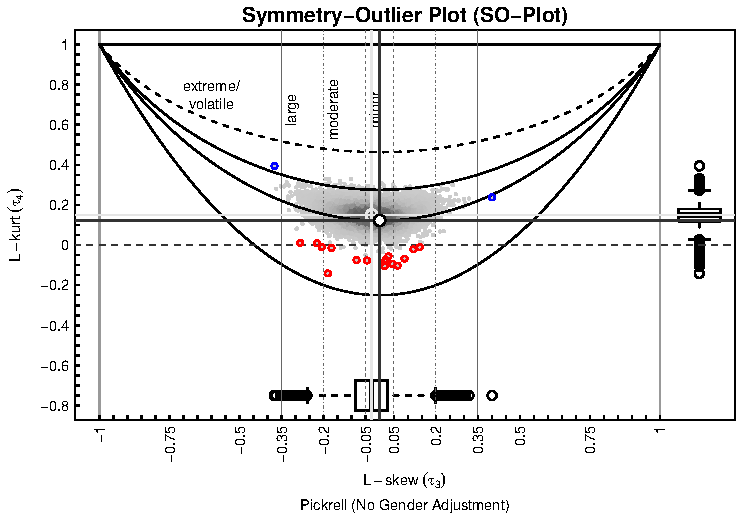
\includegraphics[width=\maxwidth]{figure/soplotPickrell-1} 

}



\end{knitrout}

\noindent Let us take a closer look at the genes called
outliers. Keep in mind that outlier here means 
that the shape of the gene 
is different from the majority of gene shapes
in the data; independent of the gene's variance and 
expression level.  
First we begin with the redGroup (contains 16 genes).

\begin{knitrout}\small
\definecolor{shadecolor}{rgb}{0.969, 0.969, 0.969}\color{fgcolor}

{\centering 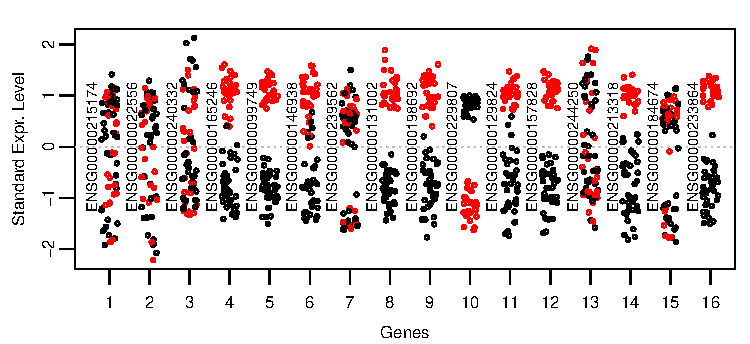
\includegraphics[width=\maxwidth]{figure/redGroupPickrell-1} 

}



\end{knitrout}

\noindent As we can see some of these genes
exhibit two groups. 
The genes are colored by sex. 
Black is female and red is male. 
Genes 4, 5, 6, 8, 9, 10, 11, 12, 14, and 16 
probably form two groups due to gender differences.
Genes 7, 13, and 15 show two groups but
probably not due to gender. 
Perhaps they are due to some
other unkown factors (biological or technical) or
they are just due to chance.
For the blueGroup

\begin{knitrout}\small
\definecolor{shadecolor}{rgb}{0.969, 0.969, 0.969}\color{fgcolor}

{\centering 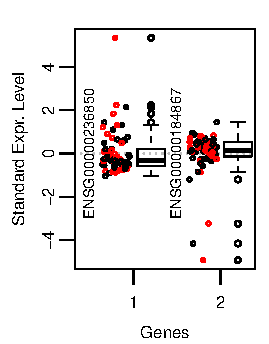
\includegraphics[width=\maxwidth]{figure/blueGroupPickrell-1} 

}



\end{knitrout}

\noindent gene 1 appears to be skewed sytematically
whereas gene 2 appears to be influenced by three 
extreme levels.

\subsection{Steps in outlier computation}
\label{outlier}

\noindent We know describe how we assign d-values to the genes.
There are three main steps:
\begin{enumerate}
\item Estimate the dependence of L-kurt $(\tau_4)$ on L-skew $(\tau_3)$ 
      with a lowess fuction.
      And ajdust the L-kurt estimates by subtracting the predicted lowess values.
\item Model the adjusted $(\tau_4)$ estimates and $(\tau_3)$ estimates 
      with a bivariate Gaussion.
      And compute the statistical distance of each point from the mean.
\item From the statistical distance obtain the exceedance probalitiy using
      a chi-square distribution with 2 degrees of freedom.    
\end{enumerate}

\noindent The backround steps can be shown when calling \texttt{computeDvals()}
by setting the argument \texttt{plot=TRUE}. 

\begin{knitrout}\small
\definecolor{shadecolor}{rgb}{0.969, 0.969, 0.969}\color{fgcolor}\begin{kframe}
\begin{alltt}
\hlstd{> }\hlkwd{head}\hlstd{(}\hlkwd{computeDvals}\hlstd{(t3, t4,} \hlkwc{plot}\hlstd{=}\hlnum{TRUE}\hlstd{))}
\end{alltt}
\end{kframe}

{\centering 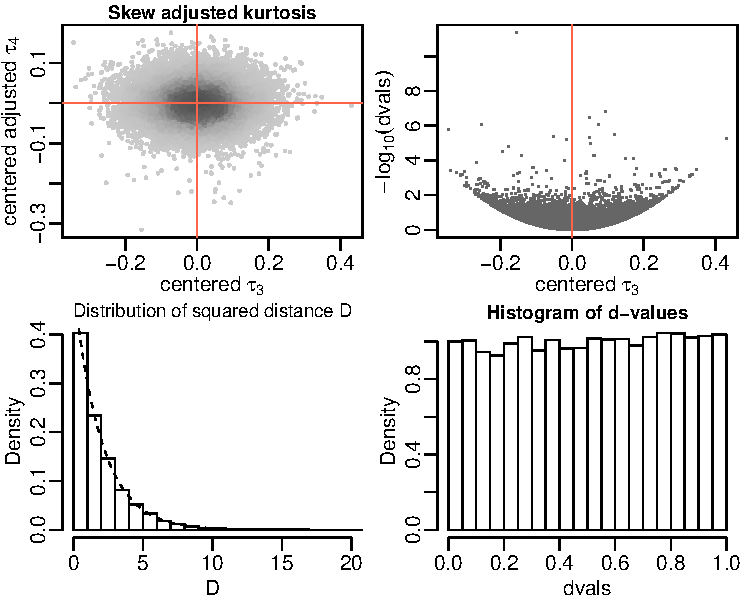
\includegraphics[width=\maxwidth]{figure/volatilePickrell-1} 

}


\begin{kframe}\begin{verbatim}
ENSG00000127720 ENSG00000242018 ENSG00000051596 ENSG00000236211 
     0.47352534      0.99400885      0.21526143      0.08799414 
ENSG00000213697 ENSG00000135541 
     0.79532942      0.74748301 
\end{verbatim}
\end{kframe}
\end{knitrout}

\noindent In the top left panel we have shown the
adjusted L-kurt and L-skew estimates (both are centered).
These points are assumed to be generated from a bivariate
Gaussian distribution. See \cite{Hosking1990} for the 
basis of this assumption. 
Statistical distances are computed for each point.
The square of these distances follow a chi-square distribution
with 2 degrees of freedom. In the bottom left panel we have
shown the histogram of the squared distances obtained from the 
Pickrell dataset. On the top of this histogram we have shown the
density of the chi-square 2-df distribution (broken curve).
The d-value for a gene is defined as the
Pr(chi-squre 2df $>$ gene's squared distance). 
In the top right panel we show the $-\hbox{log}_{10}(\hbox{d-values})$
versus the centered L-skew estimates. 
In the bottom right we show a histogram of the d-values.
Also shown are the d-values for the first 6 genes in 
the Pickrell dataset. We have called the statsitics
d-values instead of p-values in order to avoid the 
confusion that it is a formal statistical test. 
The d-value is used here as a descriptive measure.

\newpage

\section{The Hammoud dataset}

\noindent Let us now analyze the Hammoud dataset.
It contains 10 samples of mRNA profiles of 8-week 
old wild type mice (strain: C57BL/6).
Of the 10 RNA samples 5 were obtained from
spermatids (cells) and the other 5
from spermatocytes (cells).
The data has been normalized and are in 
RPKM units.

\begin{knitrout}\small
\definecolor{shadecolor}{rgb}{0.969, 0.969, 0.969}\color{fgcolor}\begin{kframe}
\begin{alltt}
\hlstd{> }\hlstd{hammoud} \hlkwb{<-} \hlstd{examplesData}\hlopt{$}\hlstd{hammoud}
\hlstd{> }\hlstd{rpkm} \hlkwb{<-} \hlstd{hammoud}\hlopt{$}\hlstd{exprs}
\hlstd{> }\hlstd{cond} \hlkwb{<-} \hlstd{hammoud}\hlopt{$}\hlstd{cond}
\hlstd{> }\hlstd{(tab} \hlkwb{<-} \hlkwd{table}\hlstd{(cond))}
\end{alltt}
\begin{verbatim}
cond
   Spermatids Spermatocytes 
            5             5 
\end{verbatim}
\end{kframe}
\end{knitrout}

\subsection{SO-plot: with and without cell type adjustment}

\noindent First we filter out genes with low 
expression by only keeping genes whose
RPKM is more than 1 in at least 5 samples
(the minimum number of samples per group).
Next we transform the RPKM to 
$\hbox{log}_2(\hbox{RPKM} + 1)$.\\

\noindent In this analysis we will look at the
shape of the genes with and without adjustment
for cell type. 
Let us denote the 
filtered log transformed RPKM with no 
cell type adjustment as \texttt{log2RPKM}.
The adjusted data is then obtained by
subtraction the group (spermatid group and 
spermatocyte group) means from the 
corresponding samples. We will denote
this data as \texttt{resids}.\\




\begin{knitrout}\small
\definecolor{shadecolor}{rgb}{0.969, 0.969, 0.969}\color{fgcolor}\begin{kframe}
\begin{alltt}
\hlstd{> }\hlkwd{par}\hlstd{(}\hlkwc{mgp}\hlstd{=}\hlkwd{c}\hlstd{(}\hlnum{1.5}\hlstd{,} \hlnum{0.5}\hlstd{,} \hlnum{0}\hlstd{),} \hlkwc{mar}\hlstd{=}\hlkwd{c}\hlstd{(}\hlnum{2.5}\hlstd{,} \hlnum{2.5}\hlstd{,} \hlnum{1}\hlstd{,} \hlnum{0.5}\hlstd{),} \hlkwc{mfrow}\hlstd{=}\hlkwd{c}\hlstd{(}\hlnum{1}\hlstd{,} \hlnum{2}\hlstd{))}
\hlstd{> }
\hlstd{> }\hlstd{res1} \hlkwb{<-} \hlkwd{fitShape}\hlstd{(}\hlkwd{t}\hlstd{(log2RPKM))} \hlcom{# Without adjustment for cell type.}
\hlstd{> }\hlstd{res2} \hlkwb{<-} \hlkwd{fitShape}\hlstd{(}\hlkwd{t}\hlstd{(resids))} \hlcom{# With adjustment for cell type.}
\hlstd{> }
\hlstd{> }\hlkwd{plotSO}\hlstd{(res1}\hlopt{$}\hlstd{lrats[}\hlstr{"LR3"}\hlstd{,], res1}\hlopt{$}\hlstd{lrats[}\hlstr{"LR4"}\hlstd{,],}
\hlstd{ }       \hlkwc{dataName} \hlstd{=} \hlstr{"Hammoud (No adjustment)"}\hlstd{)}
\hlstd{> }\hlkwd{plotSO}\hlstd{(res2}\hlopt{$}\hlstd{lrats[}\hlstr{"LR3"}\hlstd{,], res2}\hlopt{$}\hlstd{lrats[}\hlstr{"LR4"}\hlstd{,],}
\hlstd{ }       \hlkwc{dataName}\hlstd{=}\hlstr{"Hammoud (Cell type adjusted)"}\hlstd{)}
\end{alltt}
\end{kframe}

{\centering 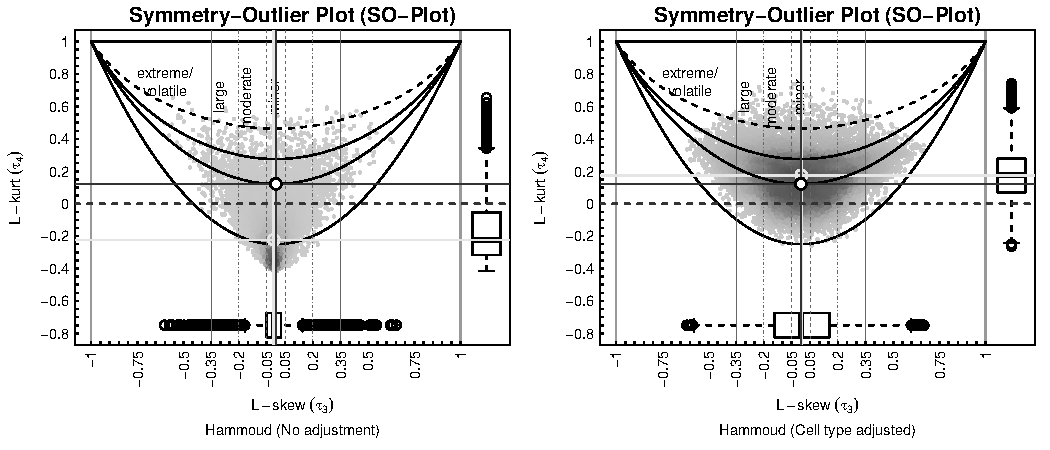
\includegraphics[width=\maxwidth]{figure/Hammoud1-1} 

}



\end{knitrout}

\noindent These two SO-plots are very different. 
The unadjusted SO-plot has the bulk of its genes below 
$\tau_4 = 0$ and concentrated at $\tau_3=0$ (symmetry). 
This suggests that a lot of genes
are differentially expressed across the cell type.
Let us investigate further by exploring the 
relationship between L-kurt and log fold change.

\begin{knitrout}\small
\definecolor{shadecolor}{rgb}{0.969, 0.969, 0.969}\color{fgcolor}

{\centering 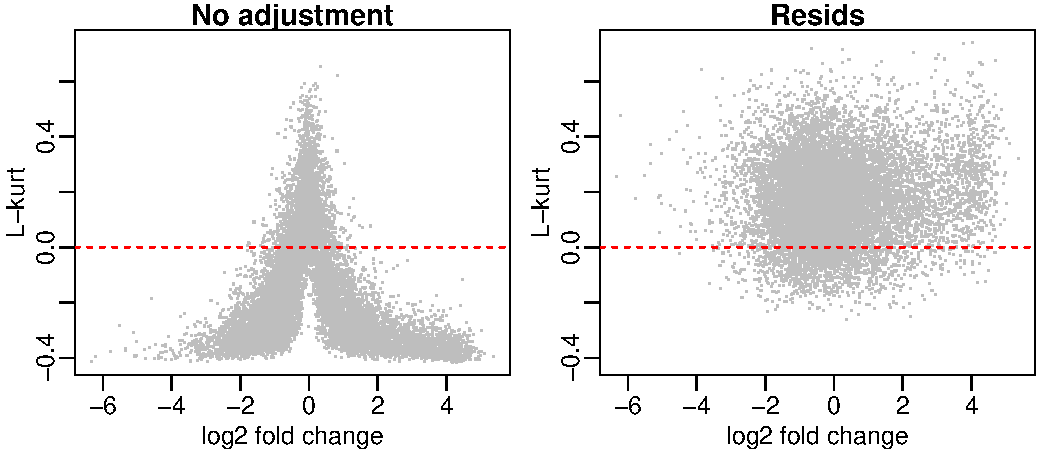
\includegraphics[width=\maxwidth]{figure/Hammoud2-1} 

}



\end{knitrout}

\noindent We can see clearly that there is a strong
relationship between L-kurt estimates and fold-change
in the No adjustment plot whereas there is none in
the Resids plot. 
Let us randomly select and plot a few (100) of the genes with
L-kurt estimates less than -0.2.
The spermatids samples are colored blue and 
the spermatocyte samples are colored red.

\begin{knitrout}\small
\definecolor{shadecolor}{rgb}{0.969, 0.969, 0.969}\color{fgcolor}

{\centering 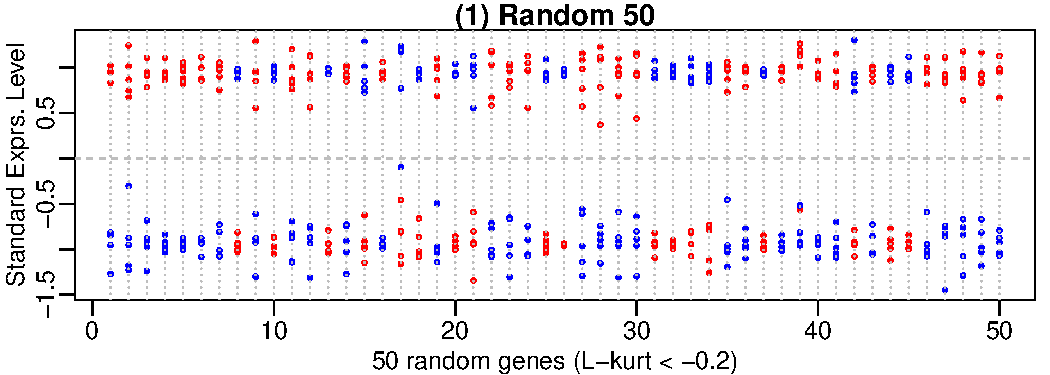
\includegraphics[width=\maxwidth]{figure/Hammoud3-1} 

}



\end{knitrout}
${}_{}$
\begin{knitrout}\small
\definecolor{shadecolor}{rgb}{0.969, 0.969, 0.969}\color{fgcolor}

{\centering 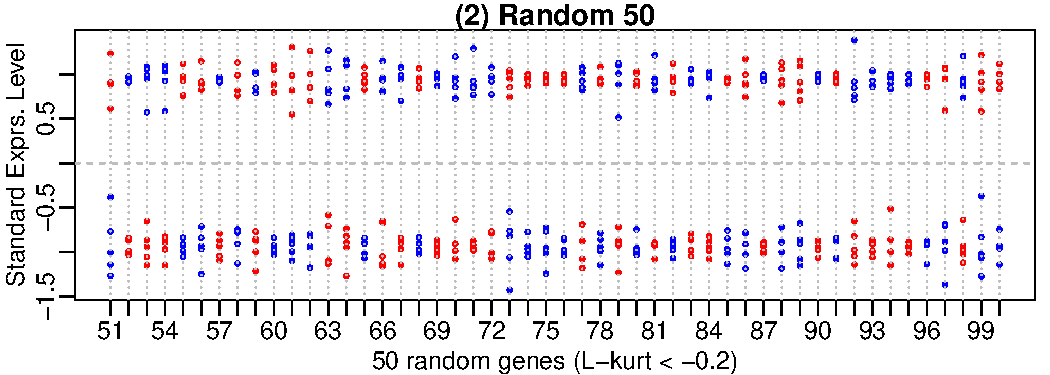
\includegraphics[width=\maxwidth]{figure/Hammoud4-1} 

}



\end{knitrout}


\newpage

\section{The Bottomly dataset}

\noindent The Bottomly dataset contains counts summarizing an RNA-seq 
experiment that includes 21 samples from inbred mouse strains.
Eleven of the samples came from the strain DBA/2J and 10 from
the strain C57BL/6J. 

\begin{knitrout}\small
\definecolor{shadecolor}{rgb}{0.969, 0.969, 0.969}\color{fgcolor}\begin{kframe}
\begin{alltt}
\hlstd{> }\hlstd{bottomly} \hlkwb{<-} \hlstd{examplesData}\hlopt{$}\hlstd{bottomly}
\hlstd{> }\hlstd{counts} \hlkwb{<-} \hlstd{bottomly}\hlopt{$}\hlstd{exprs}
\hlstd{> }\hlstd{cond} \hlkwb{<-} \hlstd{bottomly}\hlopt{$}\hlstd{cond}
\hlstd{> }\hlstd{(tab} \hlkwb{<-} \hlkwd{table}\hlstd{(cond))}
\end{alltt}
\begin{verbatim}
cond
C57BL/6J   DBA/2J 
      10       11 
\end{verbatim}
\end{kframe}
\end{knitrout}

\subsection{SO-plot: with and without strain type adjustment}

\noindent First we filter out genes with low 
expression by only keeping genes whose
cpm is more than 1 in at least 10 samples
(the minimum number of samples per condition).
Next we normalize the counts + 1 (pseudo-counts)
using DESeq's method and transform the normalized 
pseudo-counts to 
$\hbox{log}_2(\hbox{normalized pseudo-counts})$.\\

\noindent In this analysis we will look at the
shape of the genes with and without adjustment
for strain. 
Let us denote the 
filtered log transformed counts with no 
strain adjustment as \texttt{log2pcounts}.
The adjusted data is then obtained by
subtracting the group (DBA/2J group and 
C57BL/6J group) means from the 
corresponding samples. We will denote
this data as \texttt{resids}.\\




\begin{knitrout}\small
\definecolor{shadecolor}{rgb}{0.969, 0.969, 0.969}\color{fgcolor}\begin{kframe}
\begin{alltt}
\hlstd{> }\hlkwd{par}\hlstd{(}\hlkwc{mgp}\hlstd{=}\hlkwd{c}\hlstd{(}\hlnum{1.5}\hlstd{,} \hlnum{0.5}\hlstd{,} \hlnum{0}\hlstd{),} \hlkwc{mar}\hlstd{=}\hlkwd{c}\hlstd{(}\hlnum{2.5}\hlstd{,} \hlnum{2.5}\hlstd{,} \hlnum{1}\hlstd{,} \hlnum{0.5}\hlstd{),} \hlkwc{mfrow}\hlstd{=}\hlkwd{c}\hlstd{(}\hlnum{1}\hlstd{,} \hlnum{2}\hlstd{))}
\hlstd{> }
\hlstd{> }\hlstd{res1} \hlkwb{<-} \hlkwd{fitShape}\hlstd{(}\hlkwd{t}\hlstd{(log2pcounts))} \hlcom{# Without adjustment for strain.}
\hlstd{> }\hlstd{res2} \hlkwb{<-} \hlkwd{fitShape}\hlstd{(}\hlkwd{t}\hlstd{(resids))} \hlcom{# With adjustment for strain.}
\hlstd{> }
\hlstd{> }\hlkwd{plotSO}\hlstd{(res1}\hlopt{$}\hlstd{lrats[}\hlstr{"LR3"}\hlstd{,], res1}\hlopt{$}\hlstd{lrats[}\hlstr{"LR4"}\hlstd{,],}
\hlstd{ }       \hlkwc{dataName} \hlstd{=} \hlstr{"Bottomly (No adjustment)"}\hlstd{)}
\hlstd{> }\hlkwd{plotSO}\hlstd{(res2}\hlopt{$}\hlstd{lrats[}\hlstr{"LR3"}\hlstd{,], res2}\hlopt{$}\hlstd{lrats[}\hlstr{"LR4"}\hlstd{,],}
\hlstd{ }       \hlkwc{dataName}\hlstd{=}\hlstr{"Bottomly (Strain type adjusted)"}\hlstd{)}
\end{alltt}
\end{kframe}

{\centering 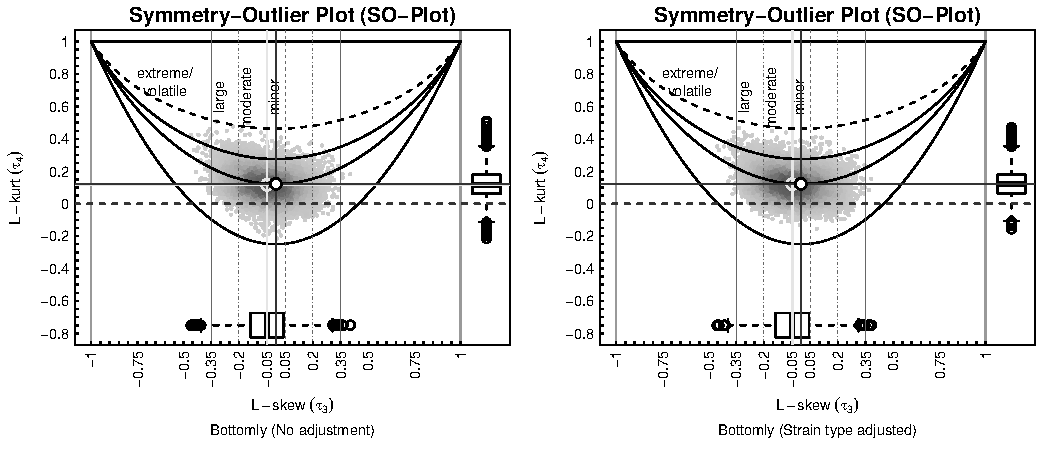
\includegraphics[width=\maxwidth]{figure/Bottomly1-1} 

}



\end{knitrout}

\noindent These two SO-plots are very similar. 
This suggests that most genes are not differentially expressed.
Let us investigate further by exploring the 
relationship between L-kurt and log fold change.

\begin{knitrout}\small
\definecolor{shadecolor}{rgb}{0.969, 0.969, 0.969}\color{fgcolor}

{\centering 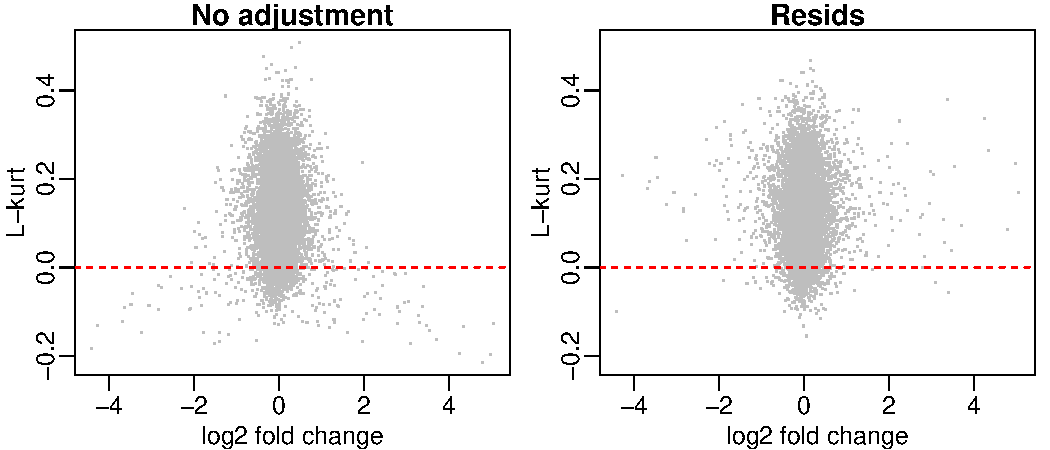
\includegraphics[width=\maxwidth]{figure/bottomly2-1} 

}



\end{knitrout}

\noindent Only a few genes change L-kurt estimates
after we adjust for strain.

\section{Shape manova}
We can use L-moments to summarize the distribution of gene expressions
for each sample. We will demonstrate this with the un-normalized 
bottomly dataset loaded from the previous section (currently defined as counts). 
Below are density plots of the first five samples.

\begin{knitrout}\small
\definecolor{shadecolor}{rgb}{0.969, 0.969, 0.969}\color{fgcolor}

{\centering 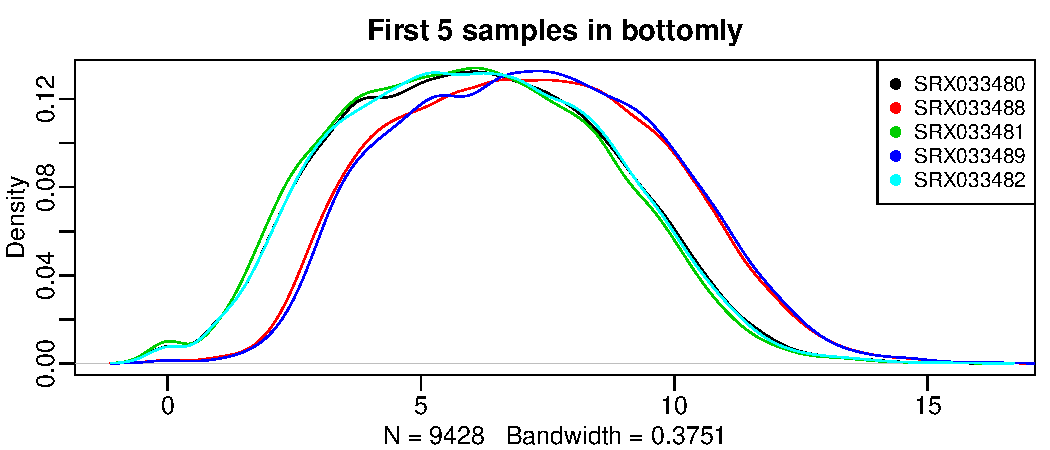
\includegraphics[width=\maxwidth]{figure/shapeManova1-1} 

}



\end{knitrout}

We can summarize the shape of these samples with L-moments statistics as
shown below.
\begin{knitrout}\small
\definecolor{shadecolor}{rgb}{0.969, 0.969, 0.969}\color{fgcolor}\begin{kframe}
\begin{alltt}
\hlstd{> }\hlkwd{fitShape}\hlstd{(}\hlkwd{log2}\hlstd{(counts}\hlopt{+}\hlnum{1}\hlstd{)[,}\hlnum{1}\hlopt{:}\hlnum{5}\hlstd{])} \hlcom{# counts equals raw counts}
\end{alltt}
\begin{verbatim}
$lcv
SRX033480 SRX033488 SRX033481 SRX033489 SRX033482 
0.2439561 0.2088938 0.2474517 0.2046416 0.2430171 

$lrats
     SRX033480  SRX033488  SRX033481  SRX033489  SRX033482
LR3 0.02298013 0.02627616 0.02389291 0.02543849 0.02255072
LR4 0.07447406 0.06760287 0.07453042 0.06876221 0.07489465

$lmoms
    SRX033480  SRX033488  SRX033481  SRX033489  SRX033482
L1 6.08659386 7.12305448 5.94364519 7.20841154 6.07479153
L2 1.48486173 1.48796205 1.47076498 1.47514057 1.47627806
L3 0.03412231 0.03909793 0.03514085 0.03752534 0.03329114
L4 0.11058368 0.10059051 0.10961673 0.10143392 0.11056534
\end{verbatim}
\end{kframe}
\end{knitrout}
\noindent Based on these statistics we can test whether the sample distributions
differ across biological groups. The shapeManova function tests this
hypothesis by performing a multivariate anova (manova) on the first four L-moments. 
It also provides single anova p-values for each L-moment separately.

\begin{knitrout}\small
\definecolor{shadecolor}{rgb}{0.969, 0.969, 0.969}\color{fgcolor}

{\centering 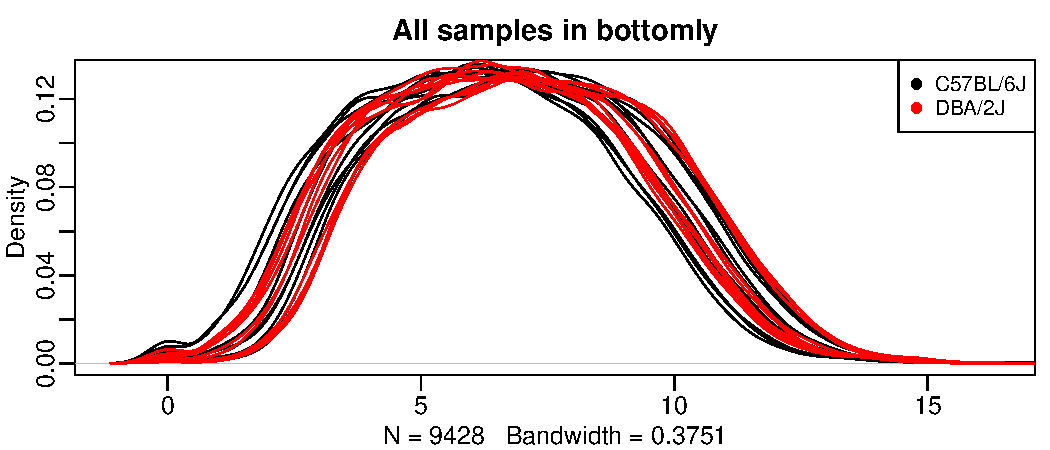
\includegraphics[width=\maxwidth]{figure/shapeManova3-1} 

}



\end{knitrout}

\begin{knitrout}\small
\definecolor{shadecolor}{rgb}{0.969, 0.969, 0.969}\color{fgcolor}\begin{kframe}
\begin{alltt}
\hlstd{> }\hlkwd{table}\hlstd{(cond)}
\end{alltt}
\begin{verbatim}
cond
C57BL/6J   DBA/2J 
      10       11 
\end{verbatim}
\begin{alltt}
\hlstd{> }\hlkwd{shapeManova}\hlstd{(}\hlkwc{data}\hlstd{=}\hlkwd{log2}\hlstd{(counts}\hlopt{+}\hlnum{1}\hlstd{),} \hlkwc{groups}\hlstd{=cond)}
\end{alltt}
\begin{verbatim}
$pvals
       L1        L2        L3        L4 
0.3730855 0.3645771 0.5002678 0.2893064 

$manova.pval
[1] 0.864
\end{verbatim}
\end{kframe}
\end{knitrout}
\noindent Individually, all the L-moments are not significantly different across the 
two mouse strains. Suggesting that the sample distributions are not significanlty
different across the mouse strains. Jointly, the manova p-value of 0.844 confirms this.

\section{Summary and discussion}

\noindent We have built on the sound 
statistical properties 
of the L-moments ratio estimators to 
provide a framework
for exploring the distributional shapes of 
genes and the detection of genes 
(volatile/outlier genes) with
shapes that are markedly different 
from the majority in a given
high-throughput
transcriptome dataset (SO-plot).
The SO-plot (symmetry-outlier) is informative 
for samples sizes as little as $n \geq 6$. 
This makes the SO-plot a very powerful tool 
for exploratory purposes.\\

\noindent Although we analyzed RNA-seq data 
other types of high-throughput data can benefit from 
this kind of analysis. In the future examples
of analyzing microarray data and methylation data
will be included in this vignette.

\section{Session Information}

\begin{knitrout}\small
\definecolor{shadecolor}{rgb}{0.969, 0.969, 0.969}\color{fgcolor}\begin{kframe}
\begin{alltt}
\hlstd{> }\hlkwd{sessionInfo}\hlstd{()}
\end{alltt}
\begin{verbatim}
R version 3.2.1 (2015-06-18)
Platform: x86_64-apple-darwin13.4.0 (64-bit)
Running under: OS X 10.10.5 (Yosemite)

locale:
[1] en_US.UTF-8/en_US.UTF-8/en_US.UTF-8/C/en_US.UTF-8/en_US.UTF-8

attached base packages:
[1] stats     graphics  grDevices utils     datasets  methods  
[7] base     

other attached packages:
[1] HTShape_1.0.0 knitr_1.12.3 

loaded via a namespace (and not attached):
[1] magrittr_1.5       formatR_1.2.1      tools_3.2.1       
[4] KernSmooth_2.23-15 stringi_1.0-1      highr_0.5.1       
[7] stringr_1.0.0      evaluate_0.8      
\end{verbatim}
\end{kframe}
\end{knitrout}

\newpage

\bibliography{HTShape}

\end{document}


